\documentclass[a4paper,11pt,twoside]{article}
%\documentclass[a4paper,11pt,twoside,se]{article}

\usepackage{UmUStudentReport}
\usepackage{verbatim}   % Multi-line comments using \begin{comment}
\usepackage{courier}    % Nicer fonts are used. (not necessary)
\usepackage{pslatex}    % Also nicer fonts. (not necessary)
\usepackage[pdftex]{graphicx}   % allows including pdf figures
\usepackage{listings}
\usepackage{pgf-umlcd}
\usepackage{blindtext}
\usepackage{enumitem}
\usepackage{amsmath}
\usepackage{amssymb}
%\usepackage{lmodern}   % Optional fonts. (not necessary)
%\usepackage{tabularx}
%\usepackage{microtype} % Provides some typographic improvements over default settings
%\usepackage{placeins}  % For aligning images with \FloatBarrier
%\usepackage{booktabs}  % For nice-looking tables
%\usepackage{titlesec}  % More granular control of sections.

% DOCUMENT INFO
% =============
\department{Department of Computing Science}
\coursename{Parallel Programming 7.5 p}
\coursecode{5DV152}
\title{Exercises, Chapter/Topic 6}
\author{Lorenz Gerber ({\tt{dv15lgr@cs.umu.se}} {\tt{lozger03@student.umu.se}})}
\date{2017-03-09}
%\revisiondate{2016-01-18}
\instructor{Lars Karlsson / Mikael Ränner}


% DOCUMENT SETTINGS
% =================
\bibliographystyle{plain}
%\bibliographystyle{ieee}
\pagestyle{fancy}
\raggedbottom
\setcounter{secnumdepth}{2}
\setcounter{tocdepth}{2}
%\graphicspath{{images/}}   %Path for images

\usepackage{float}
\floatstyle{ruled}
\newfloat{listing}{thp}{lop}
\floatname{listing}{Listing}



% DEFINES
% =======
%\newcommand{\mycommand}{<latex code>}

% DOCUMENT
% ========
\begin{document}
\lstset{language=C}
\maketitle
\thispagestyle{empty}
\newpage
\tableofcontents
\thispagestyle{empty}
\newpage

\clearpage
\pagenumbering{arabic}

\section{Introduction}
This report is part of the mandatory coursework. It describes the solutions for several chosen exercises from the course book \cite{pacheco2011}.

\section{Modification of $n$ body solver}
Yes it would be possible to remove the the inner \verb+for+ loop. However, as the calculation of force makes use of the position of all particles, updates to the position would need to be stored in a temporary variable and updated after calculating the force for all particles of the current step. This would probably deteriorate a potential speed gain from removing some structure again.

\section{Extrapolation of execution time for $n$ body solver}
The serial n-body solver was run according to the specifications in the book for 500 to 2000 particles with 3 replicates. The timings were then plotted as shown in figure \ref{fig:nbody.png}. From the plot shape, a transformation was guessed ($x^2$). Then a linear model was fitted and extrapolated to 24h. The approximation for 24h was 70'000 particles.

\begin{figure}
  \centering
  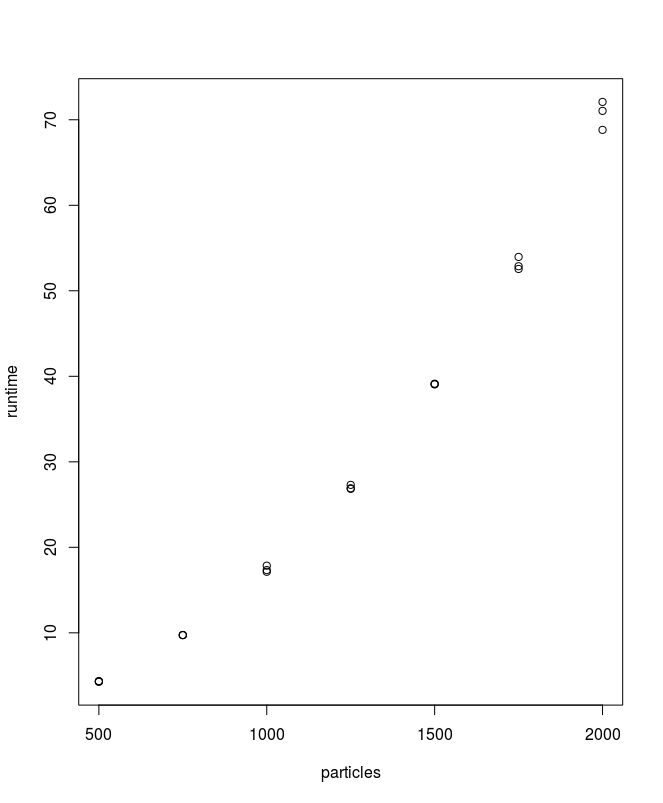
\includegraphics[width=1\textwidth]{nbody.png}
  \caption{\textit{This figure shows the measured timings from running the nbody solver with 1000 timesteps of stepsize 0.75 in range for particles from 500 to 2000. The graph was used to estimate a good transformation function. Here $x^2$ was found to be suitable }}
  \label{fig:nbody}
\end{figure}

\section{Eliminating implied barriers}
Eliminating the implied barriers in the basic OpenMP implementation has a similar consequence as described in question 6.1. As calculation of the force on particles needs the position information of each and every particle, threads that `run' ahead to the position update block and change the positions while others still calculate the force would result in wrong force values and as a consequence also false positions. Hence, removing the implied barriers would result in a wrong and unpredictable result.
  
\section{DAXPY}
Here a \textit{DAXPY} calculation was implemented using OpenMP. The source code can be seen below. The aim was to test the influence of using either a block or a cyclic partitioning for the scheduling of the parallel for loops. While cyclic partioning is obtained by using the \verb+schedule(static, 1)+ clause. For block partioning $array_length \div cores$ was used as value $n$ in the \verb+schedule(static, n)+ clause.

 The result in terms of runtimes using an increasing number of cores can be seen in figure \ref{fig:daxpy}. It is obvious that the block partitioning performs better and more consistent for all instances of core numbers. While block partioning is always faster, it's runtimes are generally also subjected to less variation compared to cyclic partitioning.

The reason for the difference in performance should be the memory access. It is much more efficient when a thread can access and use non-interrupted ranges of memory addresses as it is the case with block partioning.  
 
\begin{verbatim}
#include <stdio.h>
#include <stdlib.h>
#include "timer.h"
#include <omp.h>
#include <string.h>


int main(int argc, char *argv[]){

  double a;
  double* x;
  double* y;
  int i;
  int thread_count = strtol(argv[1], NULL, 10);
  int n = strtol(argv[2], NULL, 10);
  int c = strtol(argv[3], NULL, 10);
  
  double start, finish;

  x = malloc(n * sizeof(double));
  y = malloc(n * sizeof(double));
  
  srand(0);
  a = rand();
  for (i = 0; i < n; i++){
    x[i] = rand();
    y[i] = rand();
  }
  
  GET_TIME(start);

# pragma omp parallel private(i) num_threads(thread_count)
  {

#   pragma omp for schedule(static, c)
    for (i = 0; i < n; i++)
      x[i]=a*x[i];
#   pragma omp for schedule(static, c)
    for(i = 0; i < n; i++)
      y[i] = x[i] + y[i];
  }

  GET_TIME(finish);

  printf("%d %d %e\n", thread_count, c, (finish-start));

  free(x);
  free(y);

  return 0;
}

\end{verbatim}

\begin{figure}
  \centering
  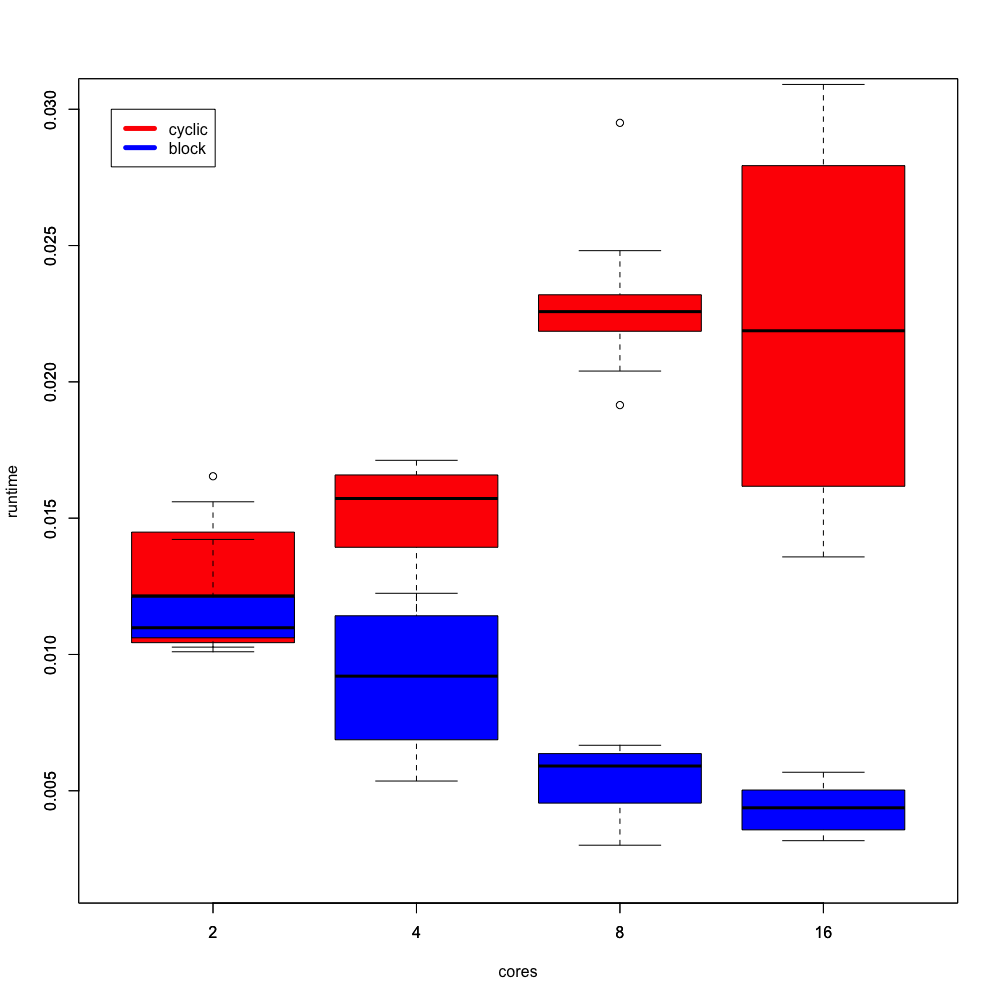
\includegraphics[width=1\textwidth]{daxpy.png}
  \caption{\textit{This figure shows the measured timings from running the omp\_daxpy.c program with either cyclic or block partitioning on 1'000'000 n arrays using $\{2, 4, 8, 16\}$ cores on the HPC2N `abisko' cluster. It is obvious that a pure cyclic scheduling is suboptimal as here threads can not work on uninterrupted ranges of memory which significantly slows down the calculation.}}
  \label{fig:daxpy}
\end{figure}

\section{L2 cache misses}
The aim here was to analyze a program consisting of two loops and determine for the second loop the number of cache misses under two different chunksizes, \verb+n/thread_count+ and \verb+8+. It is important to notice that the chunksize in the first \verb+for+ loop is \verb+n/thread_count+. In the \verb+schedule+ clause of OpenMP, this can be interpreted as block partitioning. In the current setup a cache-line holds 8 doubles and the number of doubles in the two arrays of interest are 64. Hence, in the first \verb+for+ loop each core, which by definition has it's own L2 cache, will have access to each 32 doubles in 4 cache lines (4 cache lines at each core). Using block partitioning in the first \verb+for+ loop should yield doubles of the arrays $x$ and $y$ with indices $\{0...31\}$ to end up in the L2 cache of core $0$ and those with indices $\{32...63\}$ at core $1$.

\subsection*{chunksize = n/thread\_count}
When now the schedule clause in the second \verb+for+ loop is identical to the first, it can be assumed that each core will get the indices of the loop to which there are the corresponding array entries in the L2 cache. Hence this setup results in zero cache misses.
 
\subsection*{chunksize = 8}
Here for the second \verb+for+ loop, block partitioning with chunksize 8 was chosen. As one cache line holds 8 doubles, from the total of 8 cache lines assigned during the first loop (8 per array, hence 16 for both $x$ and $y$), 4 are in the L2 of the `wrong' core. Hence, 4 cache misses per array (8 for both $x$ and $y$) will result. 

Another detail is that in this configuration, 32 doubles on 4 cache lines happen to be in the cache of the `wrong' core for the second loop. However, when a cache miss happens, a whole cache line is read again, therefore the following 7 doubles will no longer result in cache misses.  

\section{Local/global index conversions}
To devise formulas for translation from global to local indices and vice versa, the following variables are used: $k$ for rank, $b$ for blocksize, $l$ for local index and $g$ for global index.

\begin{enumerate}[label={\alph*)}]
\item global index from local for block distribution
\begin{equation*}
k \times b + l
\end{equation*}
\item local from global for block distribution
\begin{equation*}
g \mod b
\end{equation*}
\item global from local for cyclic distribution
\begin{equation*}
(g-k) \div b
\end{equation*}
\item local from global for cyclic distribution
\begin{equation*}
l \times b + k
\end{equation*}
\end{enumerate}


\section{Stack splitting in TSP}
\begin{enumerate}[label={\alph*)}]
\item Splitting the stack half, $k/2$
\item Sorting for tour length, divide round robin
\item Sorting for tour-length-divided-by-number-of-nodes, divide round robin
\end{enumerate}

All programs were implemented using the pthread `dynamic tsp' program as basis. Beside sort comparator functions, all code to be changed was within the \verb+Split_stack+ function. The source code for the \textit{k/2} implementation can be found in appendix \ref{app:k2}, for the \textit{least-cost} implementation in appendix \ref{app:cost} and for the \textit{average cost per edge} in appendix \ref{app:avgcost}.  

The implemented programs were run batch run for benchmarking on the HPC2N cluster. Each measurment was repeated five times. Looking at individual boxplots (not shown) it was obvious that variation within replicates was small, hence the data was summarized using median values in table \ref{tab:tsp}.

\begin{table}[]
\centering
\caption{\textit{This table shows the timing from running various version of the Travelling Salesman Problem algorithm. The difference between the various versions is how the stack is splitted when one thread runs out of work. Timings were collected on the HPC2N `Abisko' cluster.}}
\label{tab:tsp}
\begin{tabular}{l|cccc}
cores & dynamic & k/2   & cost  & avg cost \\ \hline
1     & 78.09   & 77.50 & 78.40 & 77.43    \\
2     & 41.13   & 41.53 & 40.79 & 40.42    \\
4     & 22.29   & 22.14 & 22.26 & 22.17    \\
8     & 12.85   & 12.95 & 12.97 & 12.67   
\end{tabular}
\end{table}


\section{Choosing an API}
\begin{enumerate}[label={\alph*)}]
\item \textbf{Memory requirements}
\item \textbf{Communications}
\item \textbf{Ease of Parallelization by OpenMP directives}
\end{enumerate}


\addcontentsline{toc}{section}{\refname}
\bibliography{references}

\end{document}
